\documentclass{standalone}
\usepackage{tikz}
\usepackage{inconsolata}

\usetikzlibrary{matrix}
\usetikzlibrary{positioning}
\usetikzlibrary{calc}

\begin{document}
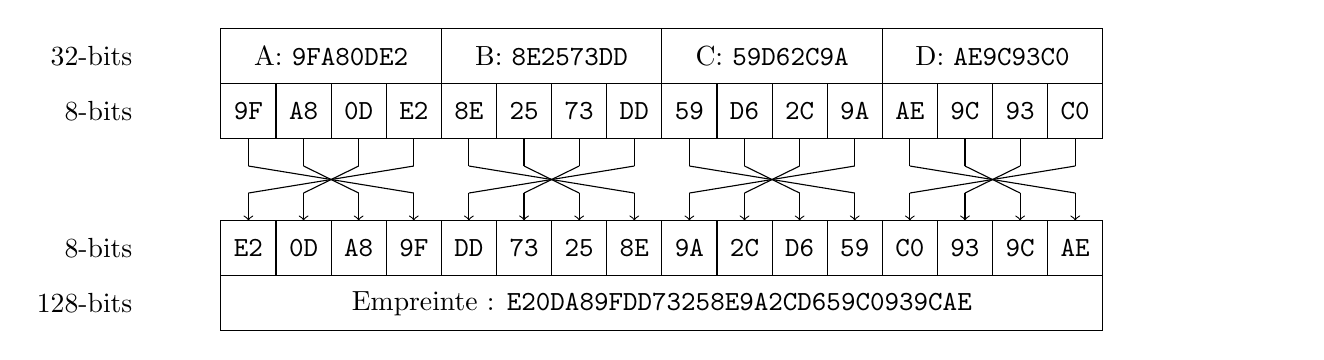
\begin{tikzpicture}
\tikzset{
int8/.style = {rectangle,draw,
               minimum width=7mm,
               minimum height=7mm,
               outer sep=0.0cm},
int32/.style = {draw,
                minimum width=28mm,
                minimum height=7mm,
                outer xsep=0.0cm},
int128/.style = {draw,
                 minimum width=112mm,
                 minimum height=7mm,
                 outer xsep=0.0cm},
table/.style = {matrix of nodes,
                row sep=3.5mm-0.5\pgflinewidth,
                column sep=-\pgflinewidth}
}

\matrix (table) [table] {
    \coordinate (A11); & \coordinate (A21); & \coordinate (A31); & \coordinate (A41);
  & \coordinate (B11); & \coordinate (B21); & \coordinate (B31); & \coordinate (B41);
  & \coordinate (C11); & \coordinate (C21); & \coordinate (C31); & \coordinate (C41);
  & \coordinate (D11); & \coordinate (D21); & \coordinate (D31); & \coordinate (D41);
  \\\node[int8] (A12) {\tt{9F}}; & \node[int8] (A22) {\tt{A8}}; & \node[int8] (A32) {\tt{0D}}; & \node[int8] (A42) {\tt{E2}};
  & \node[int8] (B12) {\tt{8E}}; & \node[int8] (B22) {\tt{25}}; & \node[int8] (B32) {\tt{73}}; & \node[int8] (B42) {\tt{DD}};
  & \node[int8] (C12) {\tt{59}}; & \node[int8] (C22) {\tt{D6}}; & \node[int8] (C32) {\tt{2C}}; & \node[int8] (C42) {\tt{9A}};
  & \node[int8] (D12) {\tt{AE}}; & \node[int8] (D22) {\tt{9C}}; & \node[int8] (D32) {\tt{93}}; & \node[int8] (D42) {\tt{C0}};
  \\\coordinate (A13); & \coordinate (A23); & \coordinate (A33); & \coordinate (A43);
  & \coordinate (B13); & \coordinate (B23); & \coordinate (B33); & \coordinate (B43);
  & \coordinate (C13); & \coordinate (C23); & \coordinate (C33); & \coordinate (C43);
  & \coordinate (D13); & \coordinate (D23); & \coordinate (D33); & \coordinate (D43);
  \\\coordinate (A14); & \coordinate (A24); & \coordinate (A34); & \coordinate (A44);
  & \coordinate (B14); & \coordinate (B24); & \coordinate (B34); & \coordinate (B44);
  & \coordinate (C14); & \coordinate (C24); & \coordinate (C34); & \coordinate (C44);
  & \coordinate (D14); & \coordinate (D24); & \coordinate (D34); & \coordinate (D44);
  \\\node[int8] (A15) {\tt{E2}}; & \node[int8] (A25) {\tt{0D}}; & \node[int8] (A35) {\tt{A8}}; & \node[int8] (A45) {\tt{9F}};
  & \node[int8] (B15) {\tt{DD}}; & \node[int8] (B25) {\tt{73}}; & \node[int8] (B35) {\tt{25}}; & \node[int8] (B45) {\tt{8E}};
  & \node[int8] (C15) {\tt{9A}}; & \node[int8] (C25) {\tt{2C}}; & \node[int8] (C35) {\tt{D6}}; & \node[int8] (C45) {\tt{59}};
  & \node[int8] (D15) {\tt{C0}}; & \node[int8] (D25) {\tt{93}}; & \node[int8] (D35) {\tt{9C}}; & \node[int8] (D45) {\tt{AE}};
  \\\coordinate (A16); & \coordinate (A26); & \coordinate (A36); & \coordinate (A46);
  & \coordinate (B16); & \coordinate (B26); & \coordinate (B36); & \coordinate (B46);
  & \coordinate (C16); & \coordinate (C26); & \coordinate (C36); & \coordinate (C46);
  & \coordinate (D16); & \coordinate (D26); & \coordinate (D36); & \coordinate (D46);
  \\
};

\node[int32]  at ($(A21)!0.5!(A31)$) (A) {A: \tt{9FA80DE2}};
\node[int32]  at ($(B21)!0.5!(B31)$) (B) {B: \tt{8E2573DD}};
\node[int32]  at ($(C21)!0.5!(C31)$) (C) {C: \tt{59D62C9A}};
\node[int32]  at ($(D21)!0.5!(D31)$) (D) {D: \tt{AE9C93C0}};
\node[int128] at ($(A16)!0.5!(D46)$) (F) {Empreinte : \tt{E20DA89FDD73258E9A2CD659C0939CAE}};

\node[left=of A]   {32-bits};
\node[left=of A12] {8-bits};
\node[left=of A15] {8-bits};
\node[left=of F]   {128-bits};
\node[right=of F]  {\phantom{128-bits}};

\draw[-] (A12) edge (A13) (A13) edge (A44) (A44) edge[->] (A45);
\draw[-] (A22) edge (A23) (A23) edge (A34) (A34) edge[->] (A35);
\draw[-] (A32) edge (A33) (A33) edge (A24) (A24) edge[->] (A25);
\draw[-] (A42) edge (A43) (A43) edge (A14) (A14) edge[->] (A15);

\draw[-] (B12) edge (B13) (B13) edge (B44) (B44) edge[->] (B45);
\draw[-] (B22) edge (B23) (B23) edge (B34) (B34) edge[->] (B35);
\draw[-] (B32) edge (B33) (B33) edge (B24) (B24) edge[->] (B25);
\draw[-] (B42) edge (B43) (B43) edge (B14) (B14) edge[->] (B15);

\draw[-] (C12) edge (C13) (C13) edge (C44) (C44) edge[->] (C45);
\draw[-] (C22) edge (C23) (C23) edge (C34) (C34) edge[->] (C35);
\draw[-] (C32) edge (C33) (C33) edge (C24) (C24) edge[->] (C25);
\draw[-] (C42) edge (C43) (C43) edge (C14) (C14) edge[->] (C15);

\draw[-] (D12) edge (D13) (D13) edge (D44) (D44) edge[->] (D45);
\draw[-] (D22) edge (D23) (D23) edge (D34) (D34) edge[->] (D35);
\draw[-] (D32) edge (D33) (D33) edge (D24) (D24) edge[->] (D25);
\draw[-] (D42) edge (D43) (D43) edge (D14) (D14) edge[->] (D15);
\end{tikzpicture}
\end{document}